\chapter{Grundlagen}
\label{sec:fundamentals}
\section{A* Algorithmus}
\label{sec:fundamentalsA*}
Der A*-Algorithmus ist ein Wegfindungs-Algorithmus, der von Peter Hart, Nils Nilsson und Bertram Raphael entwickelt wurde. Sein Ziel ist es den schnellsten Weg in einem Grafen vom Startknoten zum Zielknoten zu finden. 
\subsection{Funktionsweise}
\begin{wrapfigure}{r}{2.5cm}
    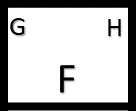
\includegraphics[width=1.5cm]{assets/aStarNode.png}
    \caption{Beispiel Node}
    \label{fig:aStarNode}
\end{wrapfigure}
Der Ausgangspunkt bildet ein zwei-dimensionales Array in dem es Felder gibt, die entweder Pfad und Hindernis darstellen. Es wird ein Start- sowie Zielfeld festgelegt. Beide sind dem Algorithmus während der Ausführung bekannt.Sobald das Spielfeld erstellt sowie ein Start- und Zielfeld gewählt wurde, sind die Mindestvoraussetzungen erfüllt. Ein Feld wird auch als Node bezeichnet und hat drei wichtige Attribute (siehe Abbildung \ref{fig:aStarNode}). Eines der Attribute sind die G-Kosten, welche die Distanz zum Start-Node darstellen bzw. die Kosten für das Beschreiten des bisherigen Wegs. Weiterhin gibt es die \textit{H-Kosten}, welche die Distanz zum Ziel darstellen. Das dritte Attribut sind die \textit{F-Kosten}. Diese werden berechnet indem man die \textit{H-Kosten} mit den \textit{H-Kosten} addiert (siehe Formel \ref{fcost}).
\begin{equation}
F_{cost} = G_{cost} + H_{cost}
\label{fcost}
\end{equation}
Für die \textit{H-Kosten} wird eine Heuristik verwendet. Hierbei wurde sich aus Simplizität für die \textit{Manhatten-Methode} entschieden. Bei dieser Methode ignoriert man den Node-Typ (Pfad oder Hindernis) und berechnet einfach die Kosten als Würde man direkt, ohne Diagonalen, zum Ziel gehen. Für die Kostenberechnung allgemein musst man sich auf einen numerischen Wert für das horizontale bzw. vertikale und diagonale Bewegung zum nächsten Node festlegen. Als Wert für die horizontale bzw. vertikale Bewegung wird 10 ($1*10$) festgelegt. Für die diagonale Bewegung wird 14 ($\sqrt{2}*10$) verwendet. Mit diesen Werten lassen sich nun die Gesamtkosten eines Nodes berechnen.

Der Algorithmus arbeitet mit zwei Listen, der \textit{Open List} und der \textit{Closed List} also die offene und geschlossene Liste. In der \textit{Open List} befinden sind die Felder, die für einen möglichen Pfad in Frage kommen. In der \textit{Closed List} sind die Nodes, welche schon beschritten wurden.

In Schritt 1 von Abbildung \ref{fig:aStarStep1_3} sind die hellblauen Felder als Start und Zielfeld markiert. Das Startfeld wird nun im zweiten Schritt (Abbildung \ref{fig:aStartStep2}) in die offene Liste aufgenommen. Von ihm werden jetzt die Nachbarn ermittelt und diese der offenen Liste hinzugefügt. Das Startfeld wird dann der geschlossenen Liste hinzugefügt, weil es jetzt als Beschritten gilt. Aus der offenen Liste wird nun das Feld mit den geringsten F-Kosten beschritten (Abbildung \ref{fig:aStartStep3}). Der Node rechts vom Start hat die geringsten Kosten, wird nun beschritten (in Lila gekennzeichnet). Dieser Node merkt sich seinen Parent, um später seinen Weg zurück verfolgen zu können. Die Parent Nodes erkennt man anhand der Pfeile, die auf sie gerichtet sind. Die Nachbarn des eben beschrittenen Nodes sind bereits in der offenen Liste, weshalb sich an dieser Liste nichts ändert.

\begin{figure}[H]
    \centering
    \begin{subfigure}[b]{0.3\textwidth}
        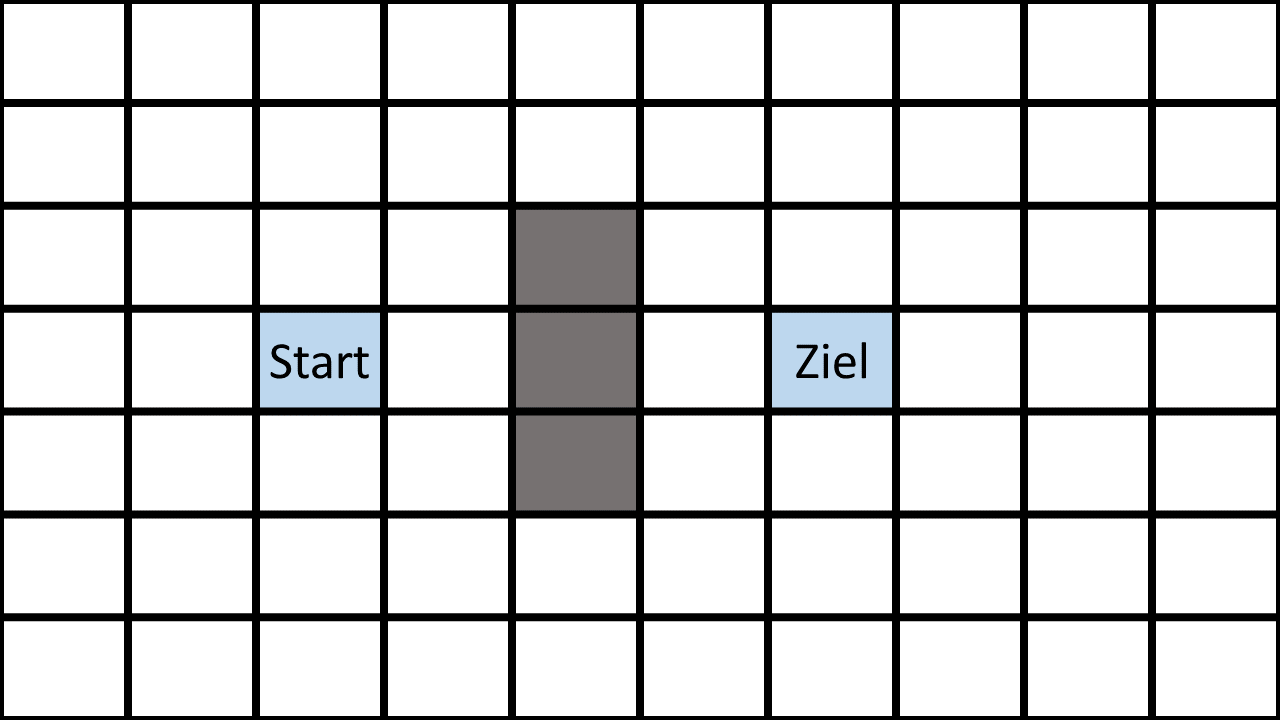
\includegraphics[width=\textwidth]{assets/aStarStep0.png}
        \caption{Schritt 1}
        \label{fig:aStartStep1}
    \end{subfigure}
    ~ %add desired spacing between images, e. g. ~, \quad, \qquad, \hfill etc. 
    %(or a blank line to force the subfigure onto a new line)
    \begin{subfigure}[b]{0.3\textwidth}
        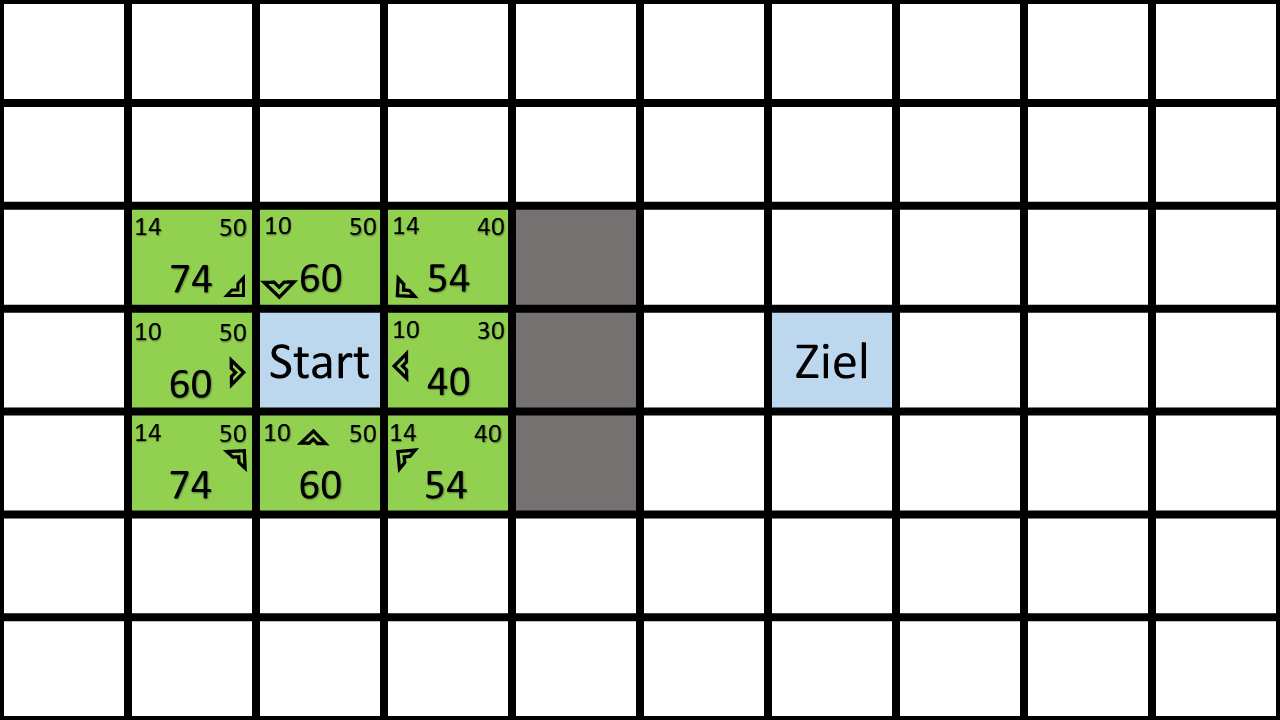
\includegraphics[width=\textwidth]{assets/aStarStep1.png}
        \caption{Schritt 2}
        \label{fig:aStartStep2}
    \end{subfigure}
    ~
    \begin{subfigure}[b]{0.3\textwidth}
        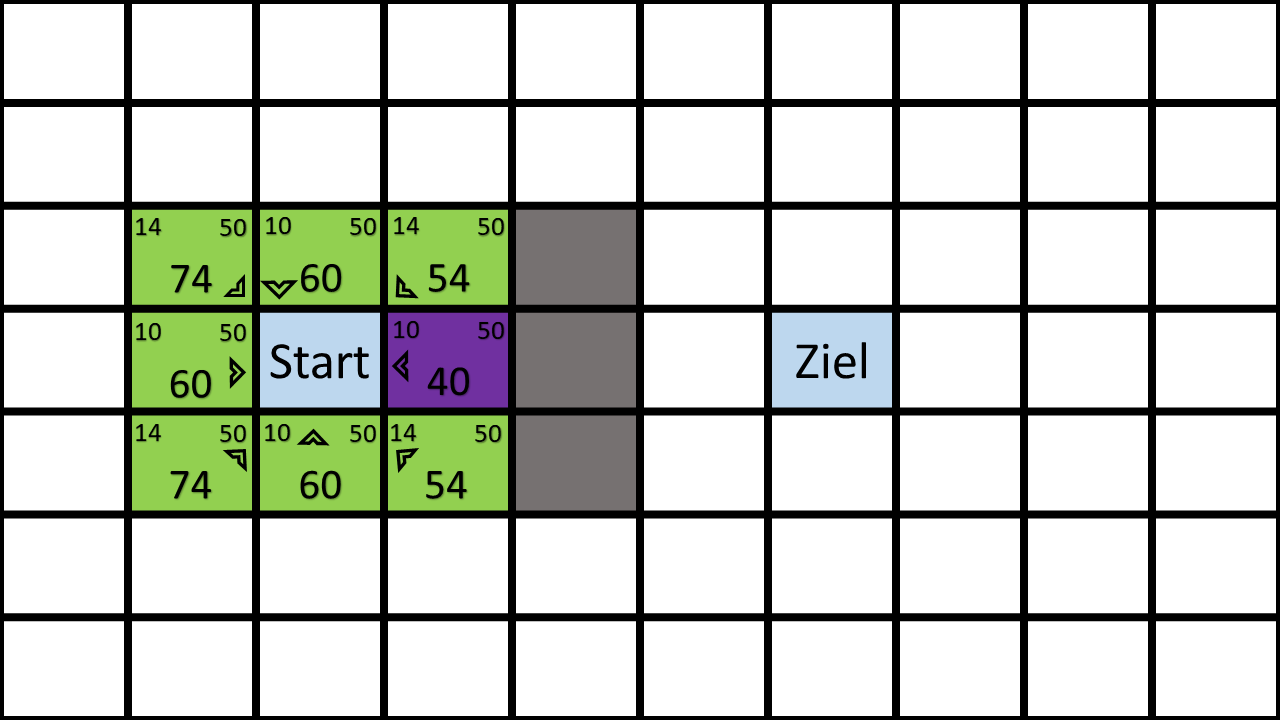
\includegraphics[width=\textwidth]{assets/aStarStep2.png}
        \caption{Schritt 3}
        \label{fig:aStartStep3}
    \end{subfigure}
    \caption{A* Ausführungsschritte 1-3}\label{fig:aStarStep1_3}
\end{figure}

Nun wird wieder der Node mit den geringsten Kosten gewählt. Er wird in die geschlossene Liste aufgenommen und seine Nachbar werden zur offenen Liste hinzugefügt Schritt 1 von Abbildung \ref{fig:aStarStep4_6}. Dieser Vorgang wiederholt sich nun neun weitere Male ( siehe Abbildung \ref{fig:aStarStep7_9}, \ref{fig:aStarStep10_12} und \ref{fig:aStarStep13}). 
\begin{figure}[H]
    \centering
    \begin{subfigure}[b]{0.3\textwidth}
        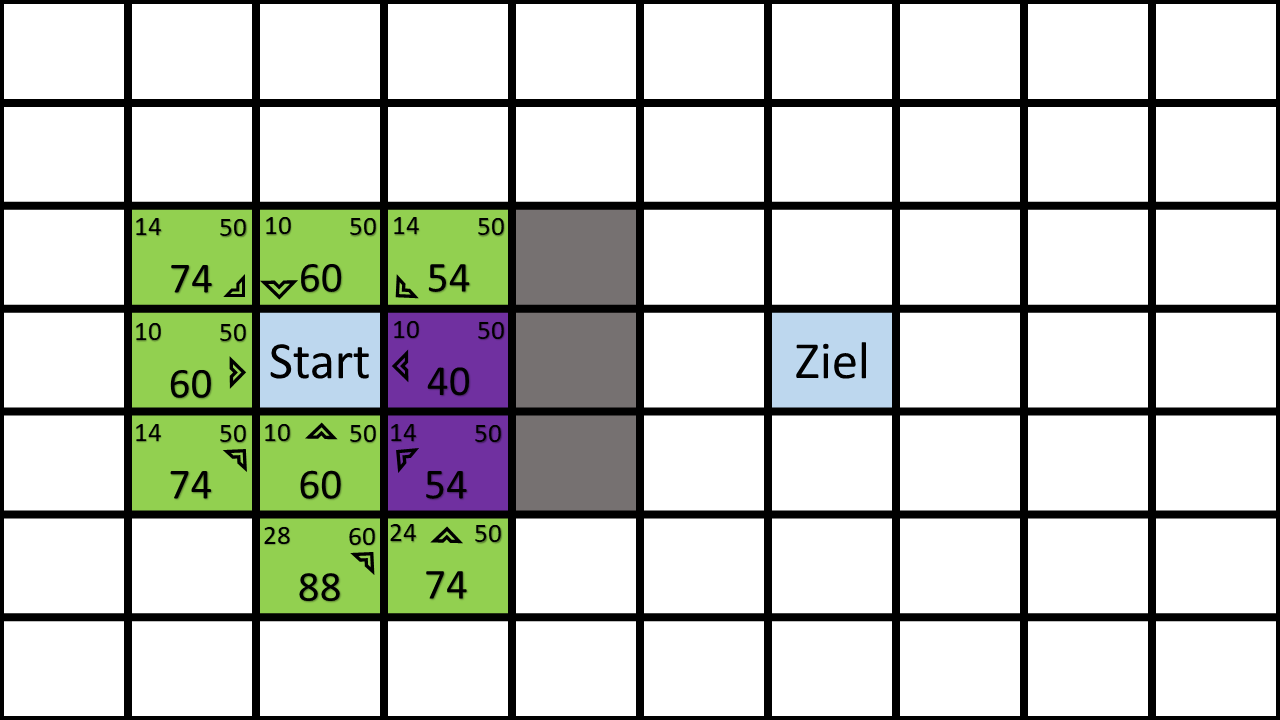
\includegraphics[width=\textwidth]{assets/aStarStep3.png}
        \caption{Schritt 4}
        \label{fig:aStartStep4}
    \end{subfigure}
    ~
    \begin{subfigure}[b]{0.3\textwidth}
        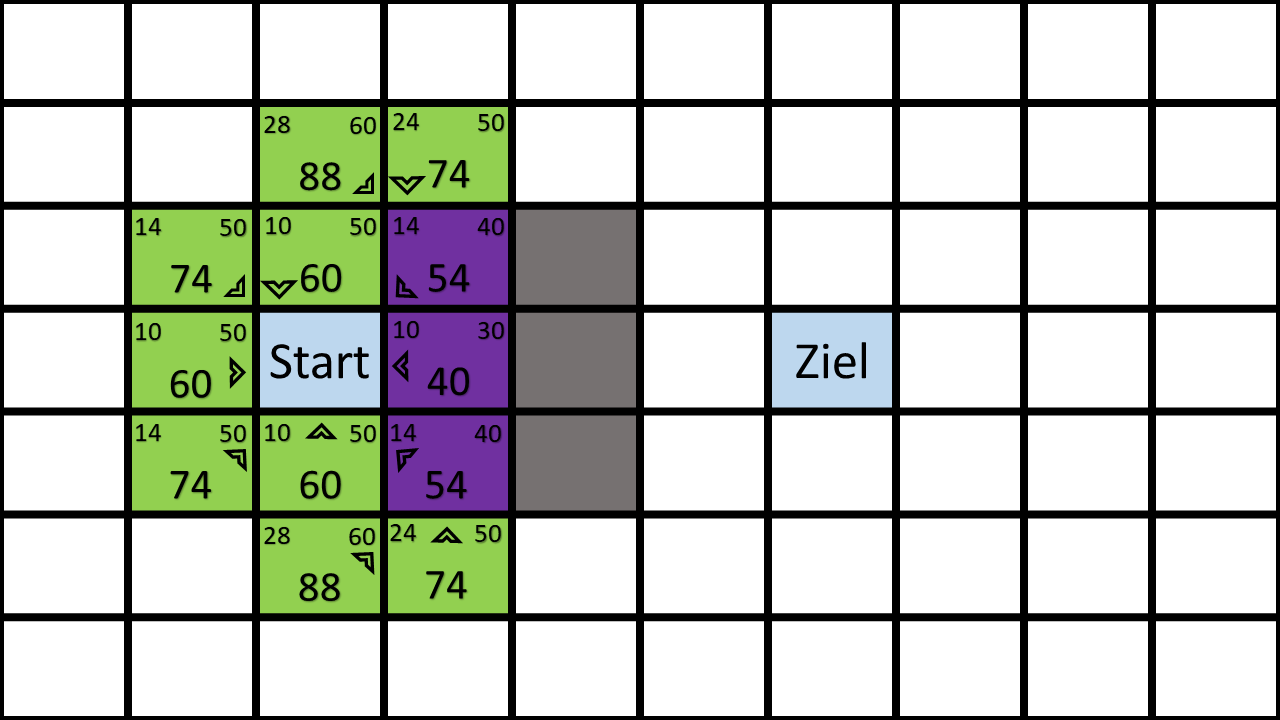
\includegraphics[width=\textwidth]{assets/aStarStep4.png}
        \caption{Schritt 5}
        \label{fig:aStartStep5}
    \end{subfigure}
    ~
    \begin{subfigure}[b]{0.3\textwidth}
        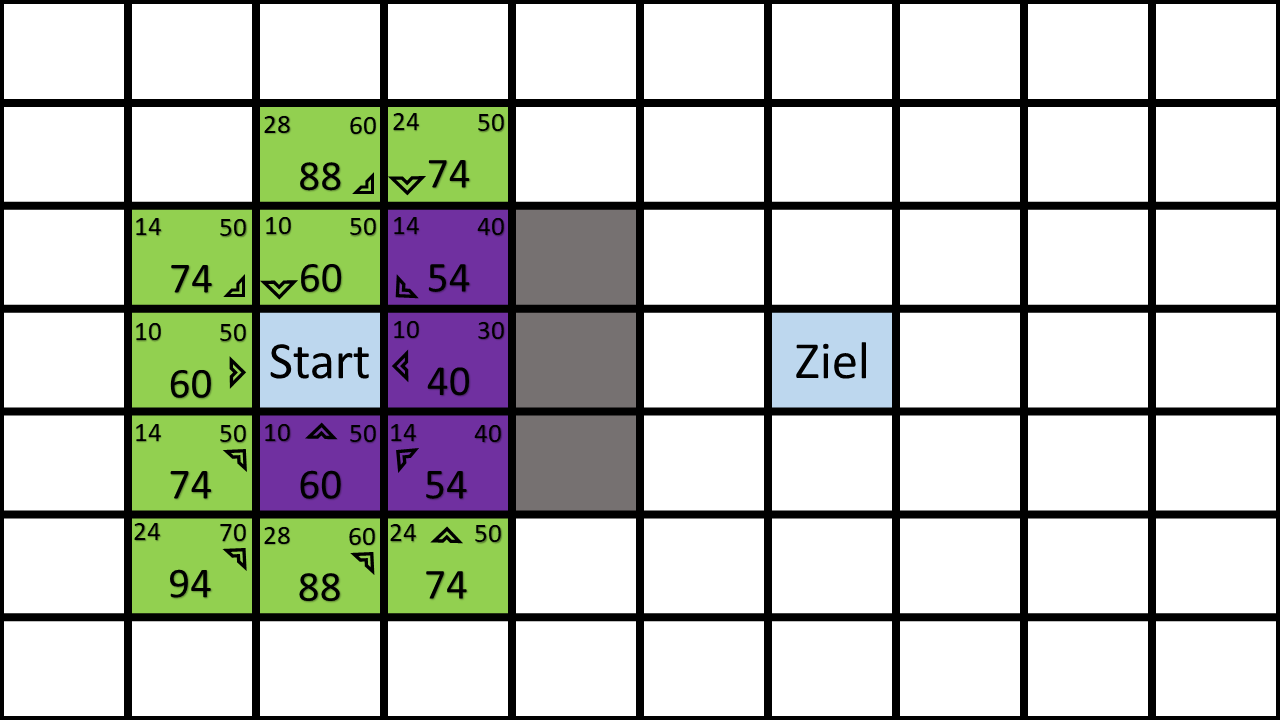
\includegraphics[width=\textwidth]{assets/aStarStep5.png}
        \caption{Schritt 6}
        \label{fig:aStartStep6}
    \end{subfigure}
    \caption{A* Ausführungsschritte 4-6}\label{fig:aStarStep4_6}
\end{figure}

\begin{figure}[H]
    \centering
    \begin{subfigure}[b]{0.3\textwidth}
        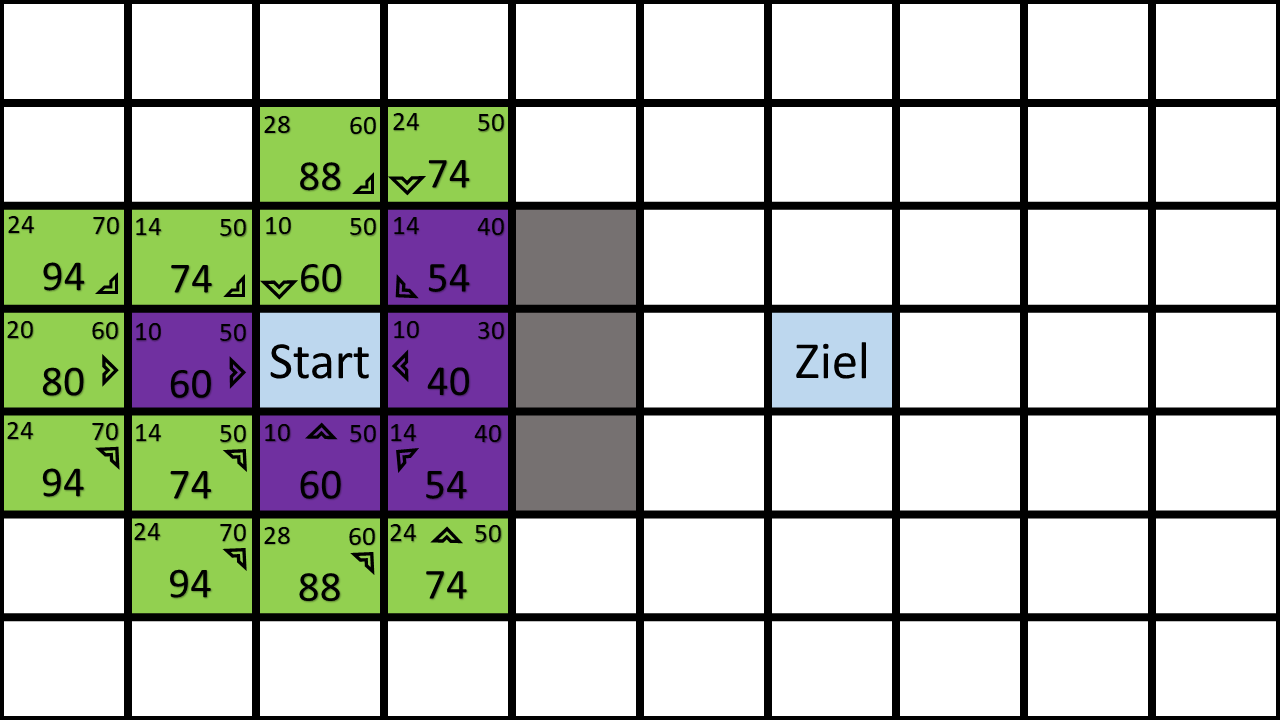
\includegraphics[width=\textwidth]{assets/aStarStep6.png}
        \caption{Schritt 7}
        \label{fig:aStartStep7}
    \end{subfigure}
    ~
    \begin{subfigure}[b]{0.3\textwidth}
        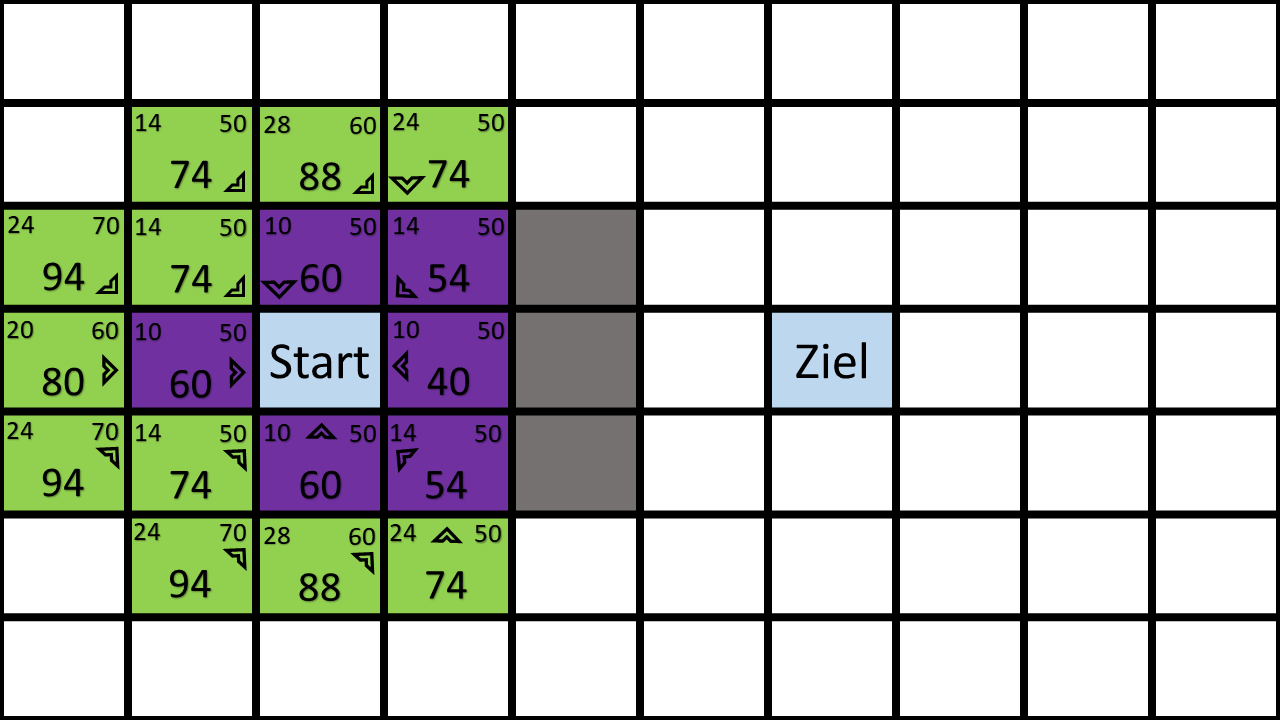
\includegraphics[width=\textwidth]{assets/aStarStep7.png}
        \caption{Schritt 8}
        \label{fig:aStartStep8}
    \end{subfigure}
    ~
    \begin{subfigure}[b]{0.3\textwidth}
        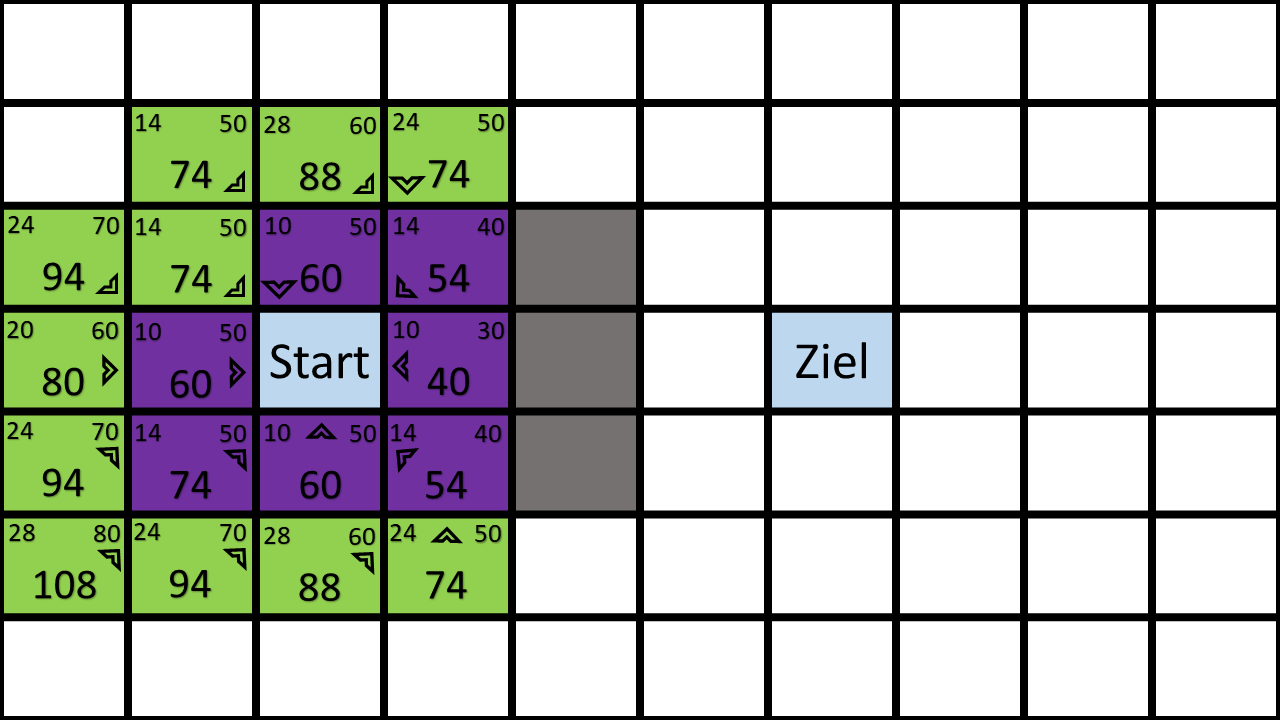
\includegraphics[width=\textwidth]{assets/aStarStep8.png}
        \caption{Schritt 9}
        \label{fig:aStartStep9}
    \end{subfigure}
    \caption{A* Ausführungsschritte 7-9}\label{fig:aStarStep7_9}
\end{figure}

\begin{figure}[H]
    \centering
    \begin{subfigure}[b]{0.3\textwidth}
        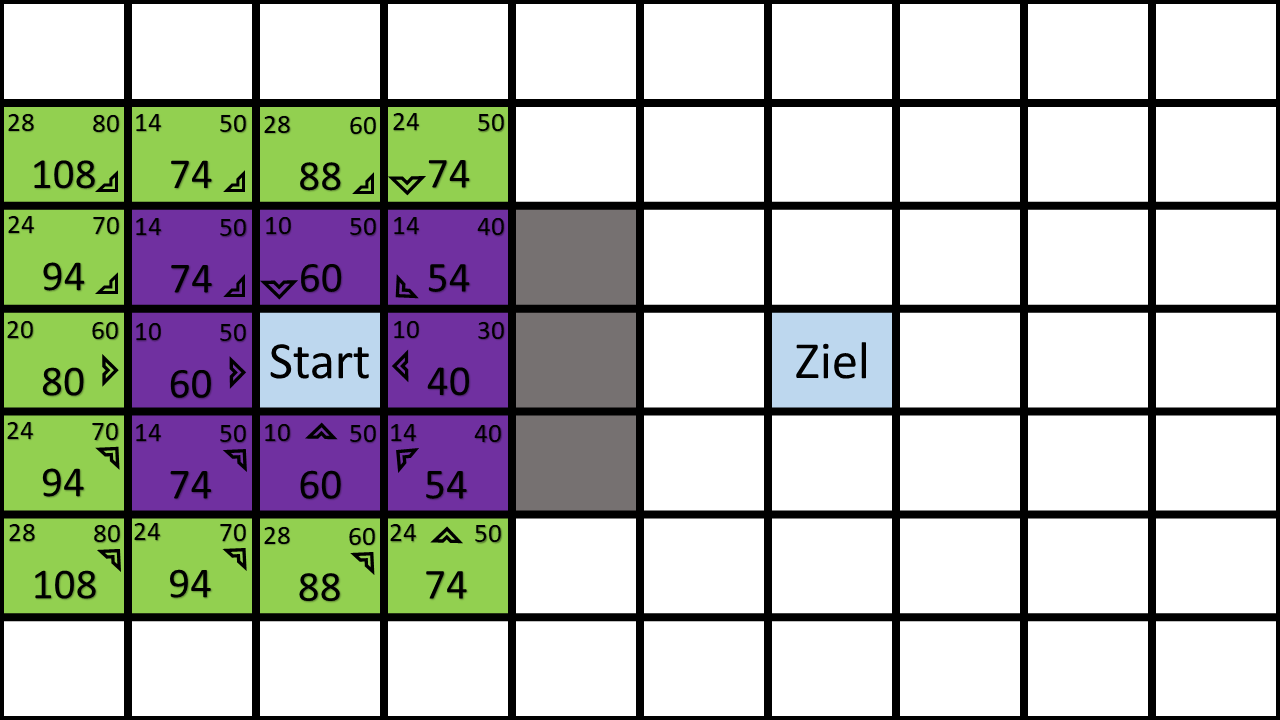
\includegraphics[width=\textwidth]{assets/aStarStep9.png}
        \caption{Schritt 10}
        \label{fig:aStartStep10}
    \end{subfigure}
    ~
    \begin{subfigure}[b]{0.3\textwidth}
        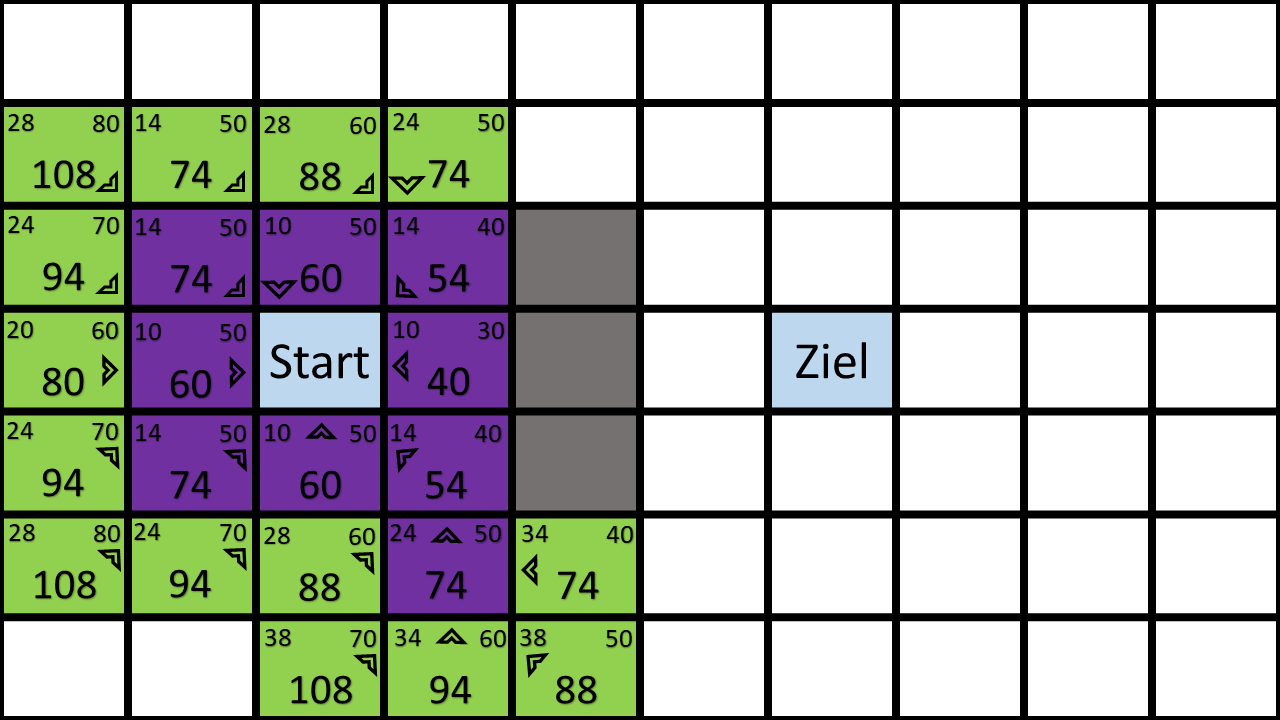
\includegraphics[width=\textwidth]{assets/aStarStep10.png}
        \caption{Schritt 11}
        \label{fig:aStartStep11}
    \end{subfigure}
    ~
    \begin{subfigure}[b]{0.3\textwidth}
        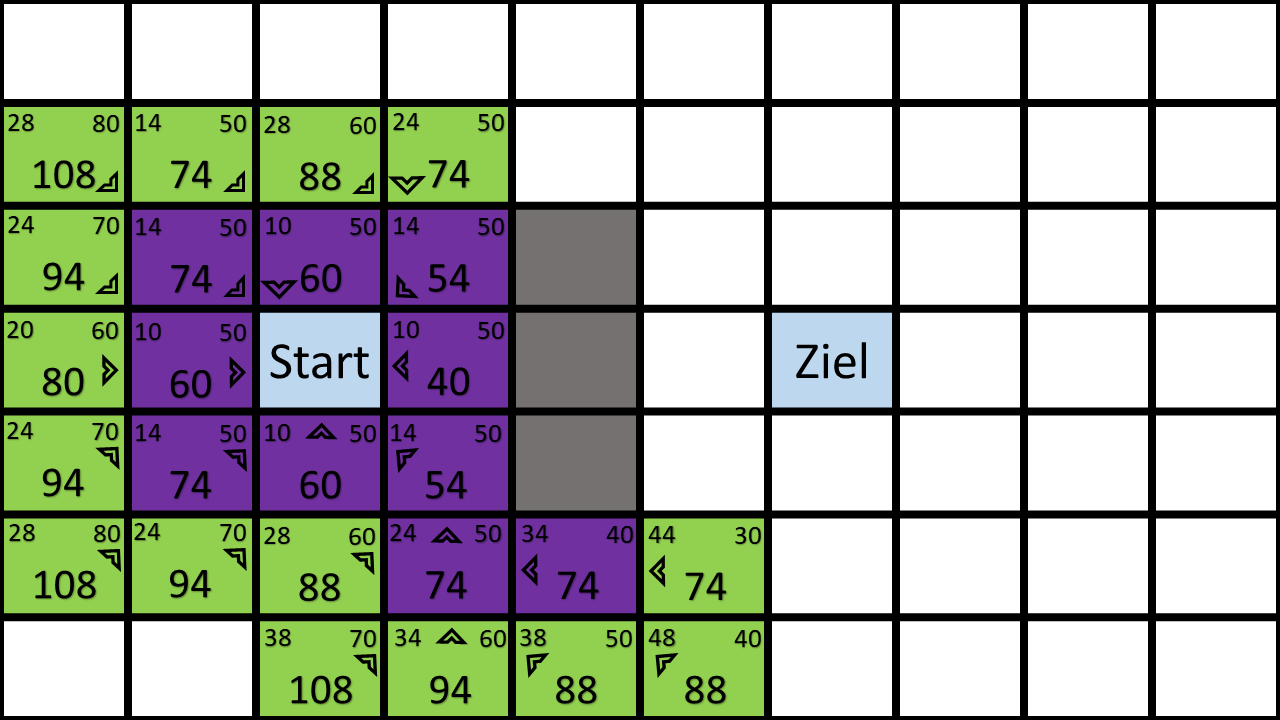
\includegraphics[width=\textwidth]{assets/aStarStep11.png}
        \caption{Schritt 12}
        \label{fig:aStartStep12}
    \end{subfigure}
    \caption{A* Ausführungsschritte 10-12}\label{fig:aStarStep10_12}
\end{figure}

Befindet sich das Ziel in der offenen Liste so ist das Ziel gefunden bzw. erreicht worden. Sollte sich kein Node mehr in der \textit{Open List} befinden gibt es keinen Pfad vom Start bis zum Ziel. Hierbei handelt es sich auch zugleich um den \textit{Worst Case}, bei dem alle Nodes besucht wurden.
Der kürzeste Pfad aus den beschrittenen Nodes kann nun mit der Zurückverfolgung anhand der Parents herausgefunden werden. Im Detail hei\ss t das, das man vom Ziel zu dessen Parent dann zum nächsten Parent usw. geht, bis man wieder auf das Startfeld trifft. Damit hat man den kürzesten Weg vom Start bis zum Ziel bestimmt. (Im \nameref{sec:anhang}, Kapitel \ref{sec:anhang}, ist eine Animation eingebettet, welche mit dem Adobe Reader abgespielt werden kann.)  
\begin{figure}[H]
    \centering
    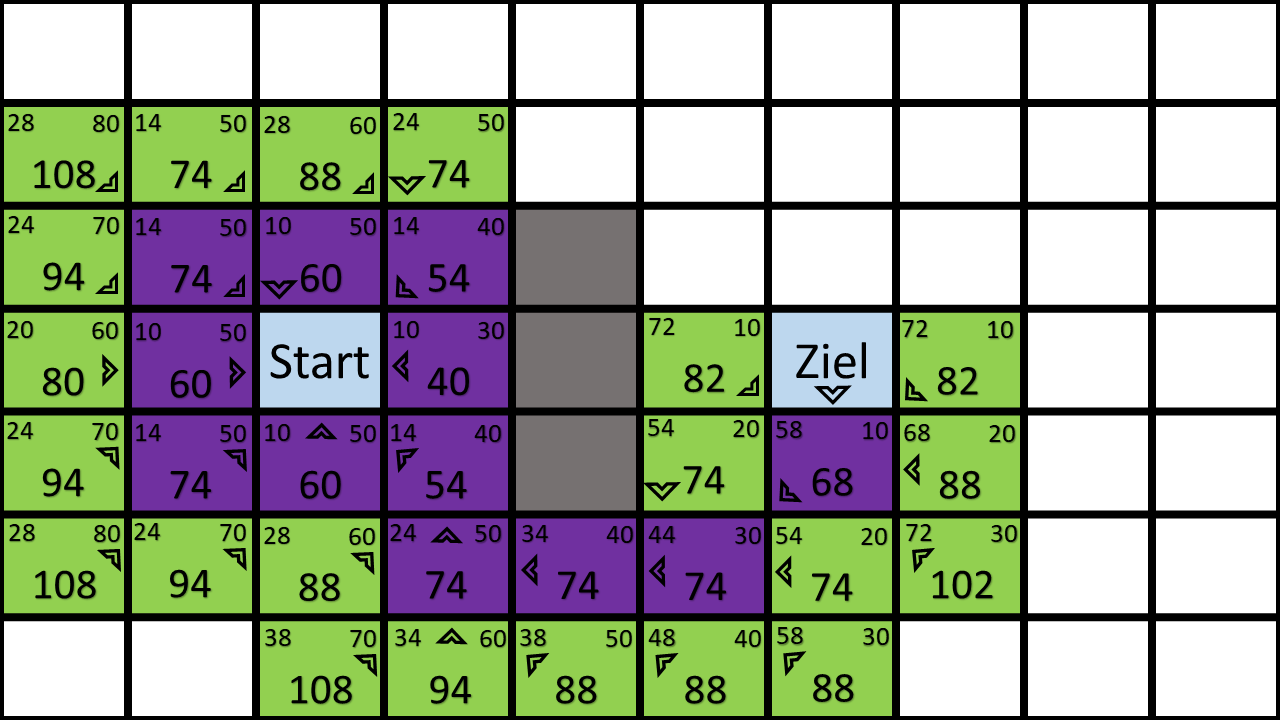
\includegraphics[width=\textwidth]{assets/aStarStep13.png}
    \caption{A* Schritt 13}\label{fig:aStarStep13}
\end{figure}
\section{Unity}

Unity ist eine Laufzeit- und Entwicklungsumgebung von \textit{Unity Technologies}. Sie eignet sich besonders gut zur Entwicklung von Spielen für unterschiedliche Endgeräte. Zielplattformen für die mit Unity entwickelt werden kann sind unter anderem Desktop Anwendungen, mobile Endgeräte und Webbrowser. So kann die GameEngine unter anderem verwendet werden um Spiele sowohl für Apples Betriebssystem iOS wie auch für Android Geräte zu builden. Unity bietet die Möglichkeit Anwendungen sowohl in 2D als auch in 3D zu entwickeln. Die Entwicklungsumgebung ist für Windows, Linux und MacOS verfügbar. \\
Die Entwicklungsumgebung erinnert an gängige 3D-Entwicklungsplattformen. Die Oberfläche besteht aus einem Hauptfenster in dem die Spielscene zu finden ist. In dieser Scene können 2D und 3D Objekte ausgewählt, skaliert und verschoben werden. Objekte in der Scene werden GameObjekt genannt und in einer hierarchisch organisierten Sidebar aufgelistet. Einem GameObjekt können weitere Komponenten wie Sounds, Materials oder Skripte zugeordnet werden. Ein einem GameObjekt zugeordnetes Skript kann das Verhalten eines GameObjekts bestimmen. Ein Skript bestimmt die Spiellogik und wird in C\# geschrieben. Der Standard Editor von Unity ist Visual Studio. Zum entwickeln kann aber auch jeder andere Editor verwendet werden. Skripte, Assets wie zum Beispiel auch 3D Modelle können als sogenannte \textit{Prefabs} zusammengefasst werden. Einem Prefab kann bestimmtes Verhalten zugeordnet werden. Dies ist von Vorteil, wenn das gleiche Objekt mehrmals in einer Scene verwendet werden soll.

\todo{Quelle: ???}

\section{Vuforia}
Bei Vuforia handelt es sich um ein Augmented Reality SDK \todo{evtl. einmal ausschreiben}[h] für mobile Endgeräte. Mit diesem SDK lassen sich Augmented Reality Anwendungen für iOS und Android entwickeln. Mit Vuforia lassen sich reale Bilder (ImageTargets)\todo{immer zusammen schreiben!}[h] und einfache 3D Objekte (3D Scans) in Echtzeit erkennen und verfolgen. Vuforia bietet dem Entwickler mehrere APIs \todo{einmal ausschreiben!!!}[h]. Darunter APIs in C++, Java, Objective C++ und als Erweiterung für Unity auch in C\#. Vuforia kann in Unity als Erweiterung die Möglichkeit der Scene eine AR-Camera hinzuzufügen und ermöglicht so eine Augmented Reality Umgebung in der Anwendung. Vuforia erweitert die Auswahl von GameObjects in Unity. Der Scene können durch Vuforia, GameObjects wie ImageTargets, ModelTargets, 3D Scans oder VuMarks hinzugefügt werden.

\todo{Quelle: https://www.vuforia.com/engine.html}

\subsection{ImageTargets}
\label{sec:fund_imagetargets}
Ein ImageTarget ist ein reales Objekt, welches von der Vuforia AR-Camera erkannt werden kann. Wird ein ImageTarget in der realen Welt vor der Kamera des mobilen Endgeräts platziert, erkennt das Vuforia SDK durch die Bilderkennung das ImageTarget. Auf dem erkannten ImageTarget können so virtuelle Objekte wie zum Beispiel 3D-Modelle platziert werden. Die Position und Orientierung des 3D-Modells richten sich hierbei nach dem erkannten ImageTarget. \todo{Image}
Ein Bild muss benötigt hierbei keine speziellen schwarz-weiß regionen wie zum Beispiel ein QR-Code. Das Bild wird mit einem, in einer Vuforia Datenbank hinterlegten Bildes, abgeglichen und so anhand seiner natürlichen Merkmale erkannt. Befindet sich das Bild im Blickwinkel der Kamera des Endgerätes, wird dieses erkannt und so lange getrackt, bis es den Blickwinkel der Kamera verlässt.\\
Bilder können im JPG oder PNG Format in RGB oder Graustufen in die Vuforia Datenbank geladen werden. Ein Bild darf hierbei nicht größer als 2MB sein. Beim upload in die Datenbank muss die Breite des Bilds in Meter angegeben werden. Die Datenbank mit den Referenzbildern kann für unterschiedliche Plattformen heruntergeladen werden. Darunter unter anderem Android Studio, xCode, Visual Studio oder Unity. Das heruntergeladene Package kann dann in der jeweiligen Plattform importiert werden.

\todo{Quelle: https://library.vuforia.com/articles/Training/Image-Target-Guide \& https://developer.vuforia.com/targetmanager/project/deviceTargetListing}

\subsection{Object Recognition}
Die Vuforia Object Recognition funktioniert ähnlich wie die Erkennung von ImageTargets. Ein reales Objekt wie zum Beispiel eine Streichholzschachtel kann anhand von bestimmten Merkmalen und eines Referenzobjektes in einer Vuforia Datenbank zur Laufzeit erkannt und verfolgt werden. Damit die Objekterkennung durch Vuforia gut funktioniert, sollte das Objekt undurchsichtig und unbeweglich sein. Die Oberfläche des Objekts sollte viele kontrastbasierte, eindeutige Merkmale aufweisen, die als Referenzpunkte bei der Erkennung dienen können.\\
Referenzobjekte, die in die Vuforia Datenbank geladen werden können, müssen mit dem Vuforia Object Scanner \todo{Quelle: https://library.vuforia.com/articles/Training/Vuforia-Object-Scanner-Users-Guide} erstellt werden. Der Scanner ist eine Applikation für Android geräte, die als APK von Vuforia zur Verfügung gestellt wird. Das zu scannende Objekt wird hierbei auf einer definierten Unterlage platziert und eingescannt. Ergebnis des Scanvorgangs ist eine Object Data Datei (\textit{.od}), die in die Vuforia Datenbank geladen werden kann. Wie bei den Image Targets beschrieben, kann auch diese Datenbank heruntergeladen und in die Entwicklungsumgebung importiert werden.
